
\documentclass[12pt,a4paper,english,nofootinbib]{revtex4}
\usepackage{lmodern}
\renewcommand{\familydefault}{\rmdefault}
\usepackage[T1]{fontenc}
\usepackage[utf8]{inputenc}
\setcounter{secnumdepth}{4}
\setcounter{tocdepth}{4}
\usepackage{babel}
\usepackage{amsmath}
\usepackage{graphicx}
\usepackage{amssymb}
\usepackage{lipsum}

%\usepackage{esint}
\usepackage[unicode=true, pdfusetitle,
 bookmarks=true,bookmarksnumbered=false,bookmarksopen=false,
 breaklinks=false,pdfborder={0 0 1},backref=false,colorlinks=false]
 {hyperref}
\setlength{\oddsidemargin}{-0.25in} \setlength{\textwidth}{7.00in}
\setlength{\topmargin}{-0.25in} \setlength{\textheight}{9.0in}
\mathsurround 1.5pt
\textwidth 17cm \textheight 23 cm \oddsidemargin -0.5cm \topmargin
-1.5cm

%\input mesmacros
\def\b{\begin{equation}}
 \def\e{\end{equation}}
\newcommand{\lbl}[1]{\label{eq: #1}}
\newcommand{\rf}[1]{\ref{eq: #1}}
\newcommand{\dif}{\mathrm{d}}
\newcommand{\bq}{\begin{eqnarray*}}
\newcommand{\eq}{\end{eqnarray*}}
\newcommand{\beq}{\begin{eqnarray}}
\newcommand{\enq}{\end{eqnarray}}

\font\romdix=cmr10 \font\sldix=cmsl10 \font\bfdix=cmbx10
\newcommand{\bib}[3]{{\maj #1},\ {\romdix #2}.\ {\sldix #3}.}
\newcommand{\bibb}[4]{{\maj #1}\ {\romdix and}\
{\maj #2},\ {\romdix #3}.\ {\sldix #4}.}
\newcommand{\bibbb}[5]{{\maj #1},\, {\maj #2}\ {\romdix and}\
{\maj #3},\ {\romdix #4}.\ {\sldix #5}.}
\newcommand{\bibbbb}[6]{{\maj #1},\, {\maj #2},\, {\maj #3}\ {\romdix
and}\ {\maj #4},\ {\romdix #5}.\ {\sldix #6}.}
\newcommand{\bibbbbb}[7]{{\maj #1},\, {\maj #2},\, {\maj #3},\, {\maj #4}\
{\romdix and}\ {\maj #5},\ {\romdix #6}.\ {\sldix #7}.}
\font\maj=cmcsc10 \font\itdix=cmti10

\newcommand\dpx[1]{\frac{\partial}{\partial#1}}
\newcommand\ddpx[1]{\frac{\partial^2}{\partial#1^2}}

%\pagestyle{empty}


\newcommand\hs[1]{\hskip#1pt}
\newcommand{\sect}[1]{\setcounter{equation}{0}\section{#1}}
\renewcommand{\theequation}{\thesection.\arabic{equation}}
\newcommand{\Id}{{\bf 1}}
\newtheorem{lemma}{Lemma}
\makeatletter
%%%%%%%%%%%%%%%%%%%%%%%%%%%%%% User specified LaTeX commands.
\usepackage{latexsym}\usepackage{bm}\def\baselinestretch{1.0}




\begin{document}


\title{Generating isocurvature modes and primordial features in multi-field Higgs-$R^2$ inflation}
\author{Flavio Pineda}
%\affiliation{Physics Department, Universidad Aut\'onoma Metropolitana Iztapalapa P. O. Box 55-534, 09340 M\'exico, %CDMX., M\'exico}
\email{fpineda@xanum.uam.mx (Corresponding author}
\author{Luis O. Pimentel}
\email{lopr@xanum.uam.mx )}
    \affiliation{Departamento de Física, Universidad Aut\'onoma Metropolitana Iztapalapa P. O. Box 55-534, 09340 M\'exico, CDMX., M\'exico}
%\affiliation{}
%\author{i}
%\email{}
%\affiliation{}
\date{\today}

\begin{abstract}
\lipsum[2]
\end{abstract}

\maketitle



\section{Introduction}

La inflación cósmica se ha convertido en \lipsum[1]

A lo largo de este trabajo, usaremos la métrica de FLRW espacialmente plana

\beq 
\dif s^2 = -\dif t^2 + a^2(t) (\dif x^2 + \dif y^2 + \dif z^2)
\label{FLRW metric}
\enq 

y usamos unidades naturales tal que $c = 1$, $\hbar = 1$, $G = 1$ y $M_p = 1$.

\section{Multi-field Higgs-$R^2$ inflation}

 Nuestro punto de partida es el modelo Higgs-$R^2$ \cite{EMA2017, GORBUNOV2019, GUNDHI2020} en el marco de Jordan en su forma completa, es decir, la teoría de la inflación de Higgs \cite{BEZRUKOV2008} con un término $R^2$, cuya acción está dada por

 \beq 
    S_J[g_{\mu\nu}\,,\mathcal{H}] = \int \dif^4 x \sqrt{-g_J}\left[ \dfrac{1}{2}\left(1 + \dfrac{2\xi_h}{1}|\mathcal{H}|^2 \right) R_J + \xi_s R_J^2 - g_J^{\mu\nu}(D_\mu \mathcal{H})^\dagger (D_\nu \mathcal{H}) -\lambda|\mathcal{H}|^4 \right]\,,
 \enq 


donde las variables definidas en el marco de Jordan las denotamos con un subóíndice $J$. El campo $\mathcal{H}$ es el doblete del campo de Higgs con un acoplamiento no mínimo $\xi_h$ , necesario para que $\mathcal{H}$ produzca inflación, mientras que $\lambda$ es la constante cuártica de acoplamiento y  $D_\mu\mathcal{H}$  es la derivada covariante del sector Higgs del SM, la cual incluye las interacciones con los campos de norma 

\beq 
D_\mu\mathcal{H} = \left(\partial_\mu - \dfrac{ig}{2}\tau_a\,W^a{}_\mu  + \dfrac{ig'}{2}B_\mu\right)\mathcal{H}\,.
\enq 

Los campos $W^a_\mu$ y $B_\mu$ representan los campos de norma de los grupos $SU(2)$ y $U(1)$, con sus respectivas constantes de acoplamiento $g$ y $g'$, mientras que $\tau_a$ son los generadores de $SU(2)$. Es usual definir el doblete de Higgs $\mathcal{H}$ en la norma unitaria tal que $\mathcal{H}$ esté parametrizado por un único campo $h$

\beq 
\mathcal{H} = \dfrac{1}{\sqrt{2}}\begin{pmatrix}
    0\\
    h + v_\mathrm{ew}
\end{pmatrix}\,,
\enq 

donde $v_\mathrm{ew} \approx 246\,\mathrm{GeV}$ es la escala de energía del sector electrodébil. En esta norma, y considerando que  $M_p = 2.18 \times10^{18}\,\mathrm{GeV}\gg v_\mathrm{ew}$, la acción del modelo se puede reescribir como \cite{EMA2017}

\beq 
    S_J[g_{\mu\nu}\,,h] = \int \dif^4\sqrt{-g_J}\left[ \dfrac{1}{2}\left(1 +  \xi_h h^2\right)R_J + \xi_s R_J^2 - \dfrac{1}{2}g_J^{\mu\nu}(\partial_\mu h)(\partial_\nu h) - \dfrac{\lambda}{4}h^4  \right]\,,
    \label{Higgs-R2 action}
\enq 

donde hemos omitido las interacciones con los campos de norma. Es bien sabido que este modelo es una extensión natural del modelo de inflación de Higgs que resuelve el problema de la constante de grande de acoplamiento \cite{GORBUNOV2019}. El modelo de Higgs necesita una constante de acoplamiento  $\xi_h \sim \mathcal{O}(10^4)$ para que el modelo sea compatible con los observables del CMB; sin embargo, el modelo sufre el problema del acoplamiento fuerte \cite{Barbon2009, Burgess2009, BEZRUKOV2008}, el cual consiste en lo siguiente: el campo de Higgs se acopla fuertemente en la escala electrodébil y pierde la unitaridad perturbativa muy por debajo de la escala habitual de Planck \cite{GORBUNOV2019}. La escala de energía es $\Lambda_\text{UV} = M_p/\xi_h$, lo cual hace cuestionable las predicciones del modelo. Para $\xi_h \sim \mathcal{O}(10^4)$, la escala de energía es del orden de $\Lambda_\text{UV} \sim 10^{14}$, que es menor que la escala de energía durante la inflación. Sin embargo, la inlcusión del término $R^2$ eleva la escala de energía del modelo hasta la escala de Planck de manera natural, recuperando el carácter perturbativo del modelo \cite{EMA2017,GORBUNOV2019}. El modelo \eqref{Higgs-R2 action} presenta dos grados de libertad: el campo $h$ y un grado de libertad escalar proveniente de $R^2_J$ conocido como escalarón, donde ambos campos son dinámicos y contribuyen a la historia de la expansión del universo. Dicha dinámica se puede entender de manera más sencilla reescalando la métrica $g_{\mu\nu}$  del espacio-tiempo via una transformación conforme $\Omega^2(x)$, para que la acción \eqref{Higgs-R2 action} adopte la forma estándar Einstein-Hilbert más una acción de dos campos escalares $\phi$ y $h$ \cite{Kaiser2010a}. 

La transformación conforme que permite escribir \eqref{Higgs-R2 action} en el marco de Einstein es $\Omega^2(x) =e^{-\alpha \phi}$, con $\alpha = \sqrt{2/3}$ y $\phi$ el grado de libertad proveniente de $R^2_J$ conocido como escalarón \cite{EMA2017}. La acción resulta 


\beq 
S_J \to S_E = \int \dif^4 x\sqrt{-g}\left[\dfrac{1}{2}R - \dfrac{1}{2}g^{\mu\nu}(\partial_\mu \phi)(\partial_\nu \phi) - \dfrac{1}{2}e^{-\alpha\phi}g^{\mu\nu}(\partial_\mu h)(\partial_\nu h) - V(\phi\,,h)\right ]\,,
    \label{accion marco einstein}
\enq 

donde el potencial escalar $V(\phi\,,h)$ depende de ambos campos en el marco de Einstein, y está definido como

\beq 
V(\phi\,,h) = e^{-2\alpha\phi}\left[\dfrac{1}{16\xi_s}\left(e^{\alpha\phi} - 1 - \xi_h\,h^2 \right)^2 + \dfrac{\lambda}{4}\,h^4\right]\,.
    \label{potential Einstein}
\enq

El término cinético no canónico de $h$ define  una métrica del espacio de campos no-trivial $G_{IJ}$ con componentes no nulas

\beq 
    G_{\phi\phi} = 1\,,\quad G_{hh} = e^{-\alpha\phi}\,.
    \label{field space metric}
\enq 

Este tipo de modelos con un término cinético no canónico y dos campos escalares es bien conocido y ha sido ampliamente estudiado en la literatura \cite{Lalak2007, STAROBINSKY2001, Dimarco2003,DiMarco2005, Tolley_2010, Cremonini2011}, explorando diferentes formas sencillas del potencial inflacionario. Con esto nos referimos a potenciales inflacionarios que usualmente se pueden factorizar como suma de potenciales de un solo campo $V(\phi\,,\chi) = U(\phi) + W(\chi)$, o como producto de potenciales $V(\phi\,,\chi) = U(\phi)W(\chi)$. El potencial \eqref{potential Einstein} es más complicado en este sentido, ya que no es factorizable ni como suma ni como producto de potenciales individuales que solo dependan de $\phi$ o $h$.
Además, este modelo presenta 3 parámetros: $\lambda$, $\xi_h$ y $\xi_s$. De acuerdo con \cite{EMA2017}, existen tres casos que producen inflación en la escala de energía $\phi \gg M_p$:

\begin{enumerate}
    \item $\xi_h >0\,,\xi_s >0\,, \lambda >0$
    \item $\xi_h <0\,, \xi_s > 0\,, \lambda >0$
    \item $\xi_h <0\,, \xi_s > 0\,, \lambda < 0$
\end{enumerate}

In the three cases, the inflationary dynamics is effectively reduce to a single field one for $\xi_h \gg 1$, since the isocurvature mode is heavy enough and we can integrated out. This inflationary dynamics reduction can be seen under the valley-approach that we briefly show in the appendix \ref{appendix1}.
The former case corresponds to a mixture between Higgs field $h$ and scalaron $\phi$; the inflaton potential is given by \eqref{effective potential}.  In addition, to reproduce the CMB normalization the parameters should fulfill the condition

\beq 
    4\xi_s + \dfrac{\xi_h^2}{\lambda} \simeq 2\times 10^{9}
    \label{CMB constraint}
\enq 


In the second case, inflation is caused solely by the scalaron $\phi$, and the last one corresponds to the metastable EW vacuum. 

Por otro lado, si $\xi_s \gg \xi_h^2/\lambda$, la inflación es tipo $R^2$, mientras que en el caso contrario la inflación es impulsada predominantemente por el campo de Higgs $h$ \cite{EMA2017}. Sin embargo, si no existe ninguna jerarquía en los parámetros, se asegura que tanto $\phi$ como $h$ contribuyen a la dinámica de la inflación y a la generación de las perturbaciones para $\xi_h \gg 1$. Este caso se conoce como espacio estándar de parámetros del modelo Higgs-$R^2$, y es sabido que los efectos multi-campo están ausentes \cite{ Wang2017, GUNDHI2020}.
En este tabajo exploramos el caso $\xi_h >0\,,\xi_s >0\,, \lambda >0$ con un espacio de parámetros que cumple $\xi_h \sim \lambda \xi_s \lesssim \mathcal{O}(0.1)$ de tal manera que los modos de isocurvarura y sus características primordales no sean despreciables durante la inflación \cite{Ema_2024}. Esta condición  permite que el modo de isocurvarura no sea muy pesado para ser excitado durante la inflación, haciendo relevante su evolución para las perturbaciones primordales. El valor de los parámetros, además de ser relevantes para la generación de modos de isocurvarura, tienen un impacto en la forma del potencial \eqref{potential Einstein}. En la Fig. \ref{fig1} podemos ver la estructura del potencial para dos distintos espacios de parámetros. Para un análisis más detallado sobre la forma del potencial y sus consecuencias en las trayectorias del espacio de campos, recomendamos \cite{GUNDHI2020}.

\begin{figure}
    \centering
    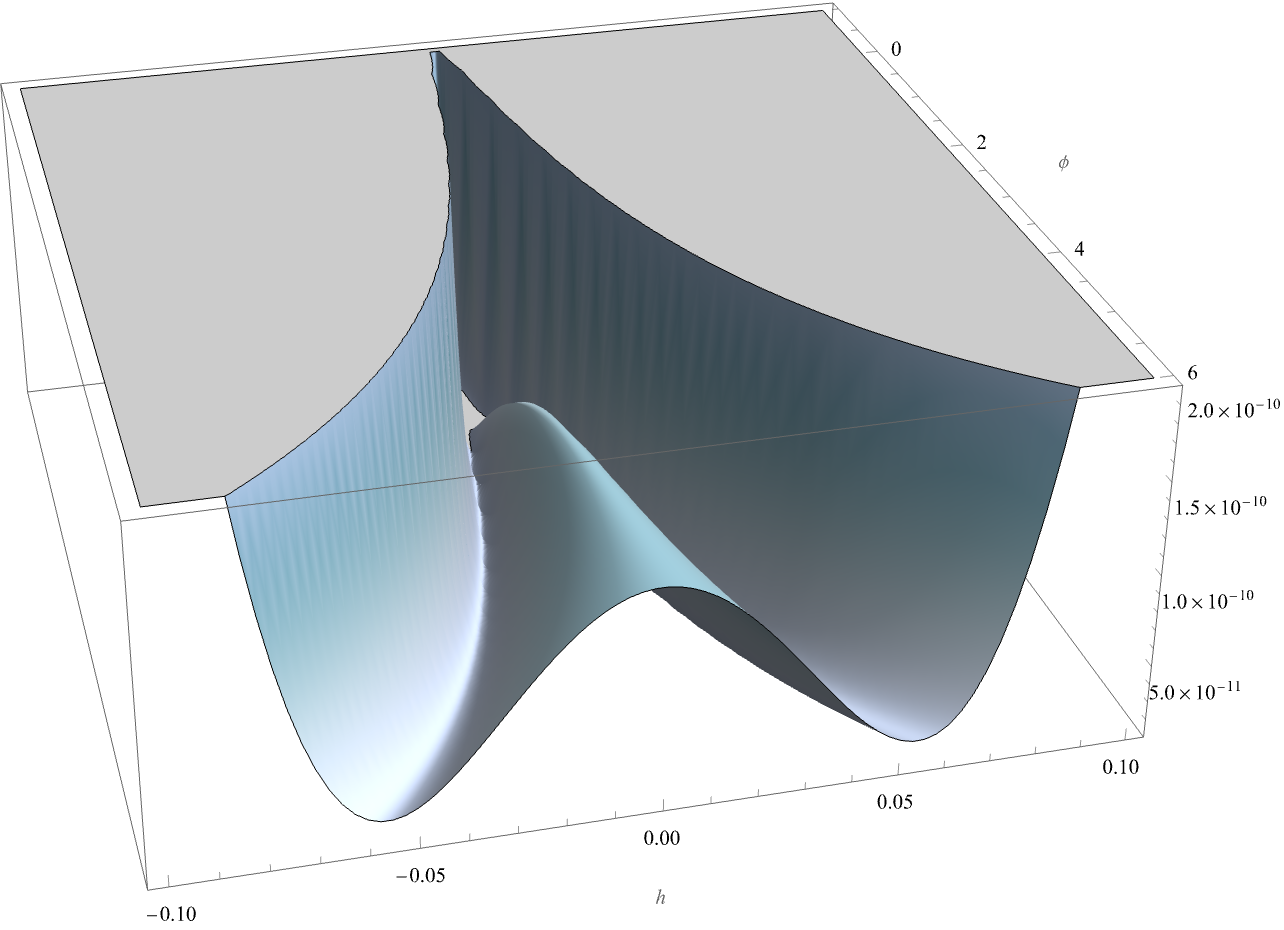
\includegraphics[width=0.48\linewidth]{Figures/potential1.png}\quad 
     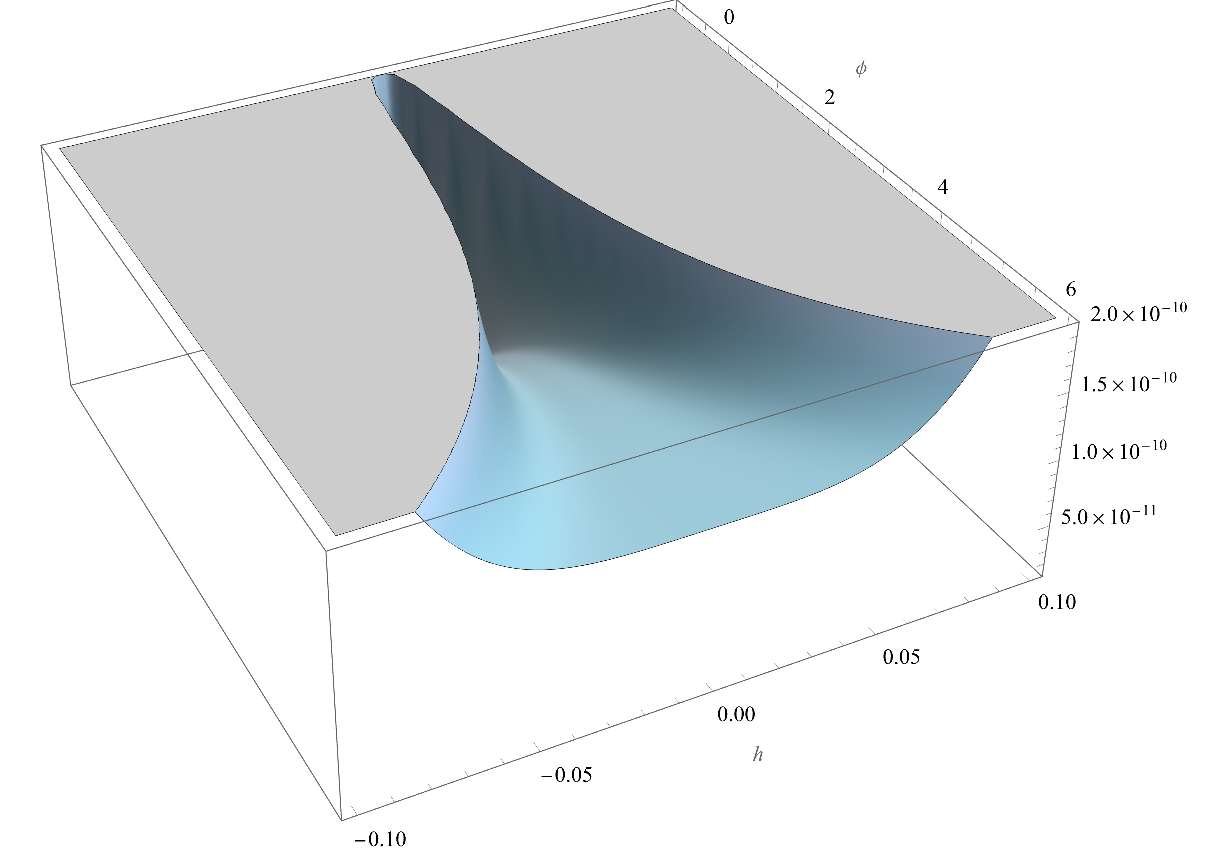
\includegraphics[width=0.48\linewidth]{Figures/potential_xi_0.3.pdf}
    \caption{Potencial escalar $V(\phi\,,h)/M_p^4$ en el marco de Einstein. Left panel: Potencial \eqref{potential Einstein} usando el espacio de parámetros estándar $\lambda = 0.13$, $\xi_h = 4000  $ y $\xi_s \simeq 10^8 $. El potencial presenta una estructura de dos valles y una cresta en $h=0$. Right panel: El mismo potencial \eqref{potential Einstein} pero para un acoplamiento $\xi_h = 0.3$. Vemos que la estructura de los valles y de la cresta del potencial desaparecen en el límite $\xi_h \ll 1$.}
    \label{fig1}
\end{figure}



\subsection{Background analysis}

Para caracterizar la evolución del sistema en modelos multi-campo de inflación, se suele utilizar un enfoque covariante  del espacio de campos  \cite{Achucarro2011, Gong2011, Gong2017, KARAMITSOS2018}. Las ecuaciones de movimiento  de los campos $\phi\,,h$ se deducen directamente de \eqref{accion marco einstein}, que usando el enfoque covariante del espacio de campos y la métrica \eqref{FLRW metric}, se escriben como

\beq 
    D_t\dot{\phi}^I + 3H\dot{\phi}^I + G^{IJ}V_J = 0\,,
    \label{EoM covariant}
\enq 


donde $D_t$ es la derivada covariante direccional en $t$, la cual se define sobre un vector arbitrario del espacio de campos $A^I$ como $D_t A^I = \dot{\phi}^J \nabla_J A^I = \dot{A}^I + \Gamma^I{}_{JK}\,\dot{\phi}^I\,A^K$, mientras que los símbolos de Christoffel están evaluados en términos de $G_{IJ}$ y sus derivadas a través de la expresión $\Gamma^I{}_{JK} = G^{IM}(\partial_J G_{KM} + \partial_K G_{JM} -\partial_M G_{JK} )/2$
, donde $\partial_J G_{KM} = \partial G_{KM}/\partial \phi^J$. Para la métrica \eqref{field space metric}, las componentes no nulas de $\Gamma^I{}_{JK}$ son 

\beq 
\Gamma^\phi{}_{h h} = \dfrac{\alpha}{2}e^{-\alpha\phi}\,,\quad \Gamma^h{}_{\phi h} = \Gamma^h{}_{h \phi} = -\dfrac{\alpha}{2}\,.
\label{Christoffel}
\enq 


En un espacio-tiempo dado por la métrica de FLRW \eqref{FLRW metric}, y suponiendo que los campos escalares son homogéneos, $\phi = \phi(t)$, $h = h(t)$, las ecuaciones de movimiento \eqref{EoM covariant} que satisfacen los campos $(\phi\,,h)$ están dadas por


\begin{align}
 \ddot{\phi} + 3H\dot{\phi} + V_\phi = -\dfrac{\alpha}{2}e^{-\alpha\phi}\dot{h}\,,\quad 
    \ddot{h} + (3H -\alpha\dot{\phi})\dot{h} + e^{\alpha\phi}\,V_h = 0\,
    \label{EoM system}
\end{align}

donde, como es usual, $\dot{} = \partial_t$, los sub-índices del potencial indican derivación y $H(t)$ es el parámetro de Hubble dado por $H= \dot{a}/a$, siendo $a(t)$ el factor de escala. La evolución y dinámica de $H$ está dado por las ecuaciones de Friedmann 

\begin{align}
\dot{H} = - \dfrac{1}{2} \dot{\sigma}^2 \,,\quad 
 3 H^2 = \dfrac{1}{2}\dot{\sigma}^2 + V(\phi\,,h)\,,
 \label{Friedmann ecs}
\end{align}


donde $\dot{\sigma}^2 = G_{IJ}\dot{\phi}^I\dot{\phi}^J =  \dot{\phi}^2 + e^{-\alpha\phi}\dot{h}^2$. La solución numérica de \eqref{EoM system}, \eqref{Friedmann ecs} con una adecuada elección de las condiciones iniciales, proporciona la trayectoria del background.  Para discutir las características de dicha trayectoria y de la geometría del espacio de campos, es útil definir los vectores tangente $T^I$ y normal $N^I$ a la trayectoria como $T^I = \dot{\phi}^I/\dot{\sigma}$ y $N^I =\sqrt{\text{det} G}\,\epsilon_{IJ} T^J$, donde $\epsilon_{IJ}$ es el símbolo de Levi-Civita totalmente antisimétrico, y $\det G$ es el determinante de la métrica \eqref{field space metric}.  De manera explícita, estos vectores para el modelo \eqref{Higgs-R2 action} están dados por 


\beq 
    T^I = \dfrac{(\dot{\phi}\,,\dot{h})}{\dot{\sigma}}\,,\quad N^I = \dfrac{e^{\alpha\phi/2}}{\dot{\sigma}}\,( -e^{-\alpha\phi}\dot{h}\,,\dot{\phi})\,.
    \label{orthogonal vectors}
\enq 


El vector $T^I$ define la dirección paralela a la trayectoria (adiabática) de cualquier vector $A^I$ del espacio de campos, mientra que $N^I$ define la primera componente normal (isocurvatura) de $A^I$. De esta manera, estos vectores nos permiten descomponer cualquier vector $A^I$ en sus componentes adiabática $A_\sigma$ y de isocurvarura $A_s$ como $A^I = A_\sigma T^I + A_s N^I$. Por otro lado, el vector $T^I$ ofrece una alternativa de escribir la ecuación de movimiento \eqref{EoM covariant} en dos ecuaciones independientes  $\ddot{\sigma} + 3H\dot{\sigma} + V_\sigma = 0$ y $D_t T^I = - H\eta_\perp N^I$, donde hemos definido $V_\sigma = T^I V_I$, $V_N = N^I V_I$ como las proyecciones de $\partial_I V = V_I$ en sus direcciones adiabática y de isocurvatura. El parámetro $\eta_\perp$ se conoce como bending e indica el cambio de $T^I$ en la dirección $N^I$.  
Si $\eta_\perp = 0$, los vectores \eqref{orthogonal vectors} permanencen covariantemente sin cambios a lo largo de la trayectoria clásica, mientras que si $\eta_\perp \neq 0$, los vectores $T^I$ y $N^I$ pueden rotar a la derecha o a la izquierda, dependiendo del signo de $\eta_\perp$. Es importante notar que si la trayectoria $\phi^I(t)$ es una geodésica en el espacio de campos $D_t \dot{\phi}^I = 0$, el bending se anula. Además, dicho parámetro es el encargado de mezclar los modos adiabático y de isocurvatura de las perturbaciones primordiales, y parametriza la interacción entre dichos modos, por lo que si tenemos movimientos geodésicos en el espacio de campos, ambas perturbaciones evolucionan de manera independiente (ver la sección \ref{perturbations}).

La caracterización de la dinámica de este tipo de modelos involucra un análisis slow-roll tal y como los modelos de inflación de un solo campo. Podemos definir los parámetros slow-roll como 

\beq 
    \epsilon = -\dfrac{\dot{H}}{H^2}\,,\quad \eta^I = - \dfrac{D_t\,\dot{\phi}^I}{H\dot{\sigma}}\,,
    \label{SR parameters}
\enq


donde $\epsilon$ es el parámetro slow-roll usual, mientras que $\eta^I$ es un vector en el espacio de campos que contiene información sobre el segundo parámetro slow-roll. Descomponemos $\eta^I$ en sus componentes adiabáticas y de isocurvarura $\eta^I = \eta_{||} T^I + \eta_\perp N^I$ donde $\eta_{||} = \eta^I T_I$ y $\eta_\perp = \eta^I N_I$ están dados por 

\beq
    \eta_{||} = -\dfrac{\ddot{\sigma}}{H\dot{\sigma}}\,, \quad \eta_\perp = \dfrac{V_N}{H\dot{\sigma}}\,.
    \label{second SR}
\enq

Es claro que la componente $\eta_{||}$ es la contraparte del segundo parámetro slow-roll de los modelos de un solo campo, mientras que $\eta_\perp$ es el bending que aparece la ecuación $D_t T^I = - H\eta_\perp N^I$. 
Las condiciones slow-roll en este tipo de modelos  están dadas por $\epsilon\ll 1\,,\quad |\eta_{||}|\ll 1$, lo cual equivale a $\ddot{\sigma} \ll |H\dot{\sigma}|$. Estas condiciones no implican un bending $\eta_\perp \ll 1$, por lo que $\eta_\perp \gtrsim 1$ es compatible con la aproximación slow-roll. Con la forma explícita de $N^I$, podemos construir la proyección de la derivada covariante del potencial \eqref{potential Einstein} en la dirección de isocurvarura

\begin{align}
    V_N = N^I V_I  = \dfrac{e^{\alpha\phi/2}}{\dot{\sigma}}(V_h \dot{\phi} - e^{-\alpha\phi}\dot{h} V_\phi)
    \label{V_N}
\end{align}

Esto permite escribir el bending del modelo como 

\beq 
\eta_\perp = \dfrac{e^{\alpha\phi/2}}{H\dot{\sigma}^2}\left( V_h \dot{\phi} - e^{-\alpha\phi}\,\dot{h}V_\phi \right)\,.
\label{bending}
\enq 

Dentro de valley-approach, el bending y los vectores ortonormales a la trayectoria del espacio de campos están dados en en \eqref{valley approach}. En el espacio de parámetros usual y dentro de valley-approach, el bending es despreciable, pero para el espacio de parámetros que cumple $\xi_h \sim \lambda\xi_s$, el bendig es del orden de $\eta_\perp \sim \mathcal{O}(0.1)$. Sin embargo, para un adecuado entendimiento de la evolución del backgrond, es conveniente hacer un análisis numérico tanto de las variables del background como de las perturbaciones. Para ello es conveniente usar el número de e-folds $N_e$ como parámetro temporal dada la relación $\dif N_e = H \dif t$. En este caso, las ecuaciones \eqref{EoM system} y \eqref{Friedmann ecs} toman la forma 

\begin{figure}[htp]
     \centering
     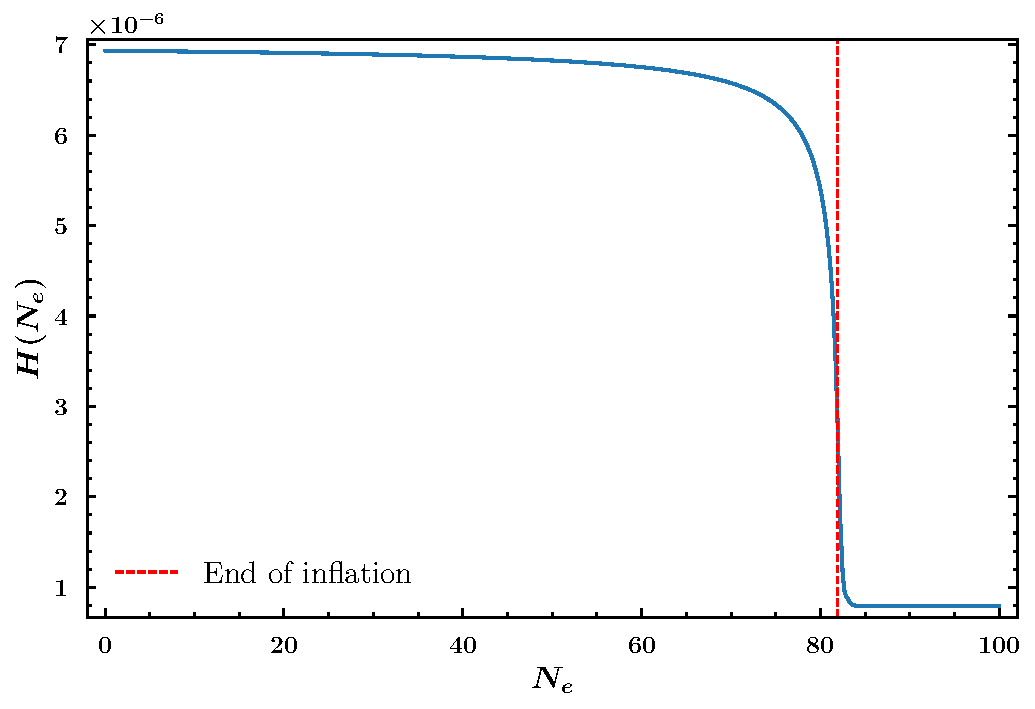
\includegraphics[width = 0.48 \textwidth]{Figures/hubbleparameter1.pdf}
     \quad
     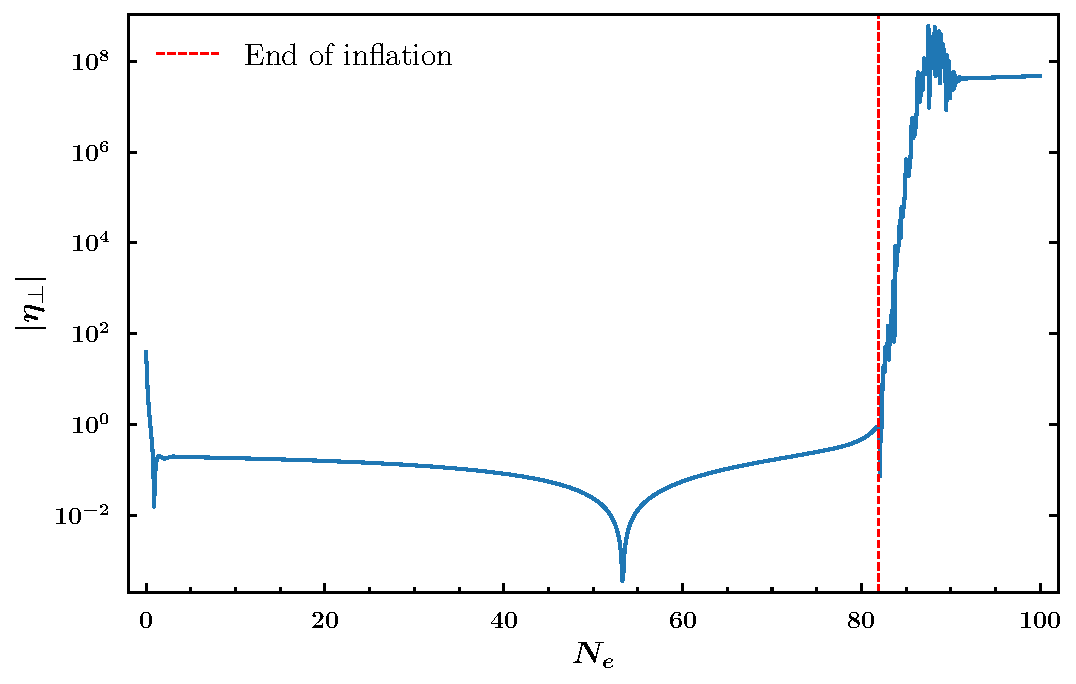
\includegraphics[width = 0.48 \textwidth]{Figures/bending1.pdf}
     \caption{Mostramos la evolución del parámetro de Hubble, $H(N_e)$, y del bending, $\eta_\perp(N_e)$, en función del número de e-folds $N_e$, obtenida al resolver las ecuaciones de fondo \eqref{efolds system}. Para ello, consideramos el espacio de parámetros $\xi_h = 0.1$, $\lambda = 10^{-10}$ y $\xi_s = 4\times10^8$ y las condiciones iniciales $\phi_0 = 5.7 M_p$, $h_0(\phi_0) = 0.096 M_p$. Se observa que el bending es del orden de $\mathcal{O}(0.1)$ y casi constante durante la inflación, lo que lo hace relevante para el análisis posterior de los modos $Q_s$.
     }
     \label{Fig2}
\end{figure}



\begin{align}
    \phi'' + (3-\epsilon)\,\phi' + \frac{V_\phi}{H^2} &= -\frac{\alpha}{2} e^{-\alpha\phi} h',\nonumber\\[0.3cm]
    h'' + (3-\epsilon-\alpha\phi')\,h' + e^{\alpha\phi}\frac{V_h}{H^2} &= 0,\nonumber\\[0.3cm]
    H^2 &= \frac{V}{3-\epsilon}\,.
    \label{efolds system}
\end{align}

donde $' = \partial_{N_e}$, mientras que el parámetro slow-roll $\epsilon$ en términos del número de e-folds se escribe como 

\beq 
    \epsilon = - \dfrac{H'}{H} = \dfrac{1}{2}(\phi'^2 + e^{-\alpha\phi}h'^2)\,,
    \label{efolds SR}
\enq

y el bending \eqref{bending} en función de $N$ está dado por 

\beq
    \eta_\perp = \dfrac{e^{\alpha\phi/2}}{\sigma_N^2}\left( V_h\phi' - e^{-\alpha\phi}\,V_\phi h' \right)\,,
    \label{bending efolds}
\enq


donde $\sigma_N^2 = H^2(\phi'^2 + e^{-\alpha\phi}h'^2)$.  Una vez que hayamos especificado los parámetros del modelo y las condiciones iniciales adecuadas, podemos proceder a integrar numéricamente el sistema de ecuaciones \eqref{efolds system} para llegar a las cantidades de fondo relevantes. Con dichas cantidades, podemos proceder a analizar las perturbaciones primordiales del modelo. 
Siguiendo a \cite{Fumagalli2021}, el análisis y evolución de la perturbaciones primordiales a orden lineal queda determinada por tres funciones: el parámetro de Hubble $H(N)$, el bending $\eta_\perp(N)$ y la masa del modo de isocurvarura $m_\text{iso}^2(N)$.
En la Fig. \ref{Fig2} mostramos la evolución del parámetro de Hubble $H(N)$ y del bending $\eta_\perp$ para el espacio de parámetros que cumple $\xi_h \sim \lambda\xi_s$. 









\section{Primordial perturbations
\label{perturbations}}

Cuando se estudia las perturbaciones primordiales a orden lineal o cuadrático en modelos multi-campo de inflación, es recomendable adoptar un enfoque covariante respecto a transformaciones de norma en el espacio de campos. Este formalismo fue desarrollado en detalle en \cite{Gong2011} para un espacio de campos arbitrario. 

En este artículo despreciamos las perturbaciones vectoriales y tensoriales, y nos enfocamos principalmente en las perturbaciones primordiales escalares. 
Desde un punto de vista covariante, la idea es utilizar la perturbación covariante $Q^I$ en lugar de $\delta\phi^I(t\,,\mathbf{r}) = \phi^I(t\,,\mathbf{r}) - \bar{\phi}^I(t)$, donde $\bar{\phi}^I(t)$ es la trayectoria clásica del background que satisface \eqref{EoM covariant}. El valor de $\bar{\phi}^I$ y $\phi^I$ en algún punto fijo $P$ del espacio de campos puede conectarse mediante una única geodésica parametrizada por un parámetro $\varepsilon$ que relaciona el valor inicial de $\phi^I$ y el vector tangente en $P$. Las condiciones iniciales se fijan en $\varepsilon = 0$, tal que


\beq 
    \phi^I (\varepsilon = 0) = \bar{\phi}^I\,,\quad Q^I = \left.\dfrac{\dif \phi^I}{\dif \varepsilon}\right|_{\varepsilon = 0} \,.
    \label{IC field space}
\enq 


 A segundo orden en las perturbaciones, uno encuentra el desarrollo que relaciona $Q^I$ con la perturbación $\delta\phi^I$


\beq 
    \delta\phi^I = \phi^I-\bar{\phi}^I = Q^I - \dfrac{1}{2}\,\Gamma^I{}_{JK}\,Q^
    JQ^K  + \cdots\,.
    \label{inflationary perturbation}
\enq 

Dado que tanto $\delta\phi^I$ como $Q^I$ son vectores del espacio de campos, podemos descomponerlos en sus componentes adiabática $Q_\sigma$ y de isocurvatura $Q_s$ como $Q^I = Q_\sigma T^I+ Q_s N^I$, donde a priori ambas componentes son dinámicas. Por otro lado, el estudio de las perturbaciones del espacio-tiempo y la mezcla con $Q^I$ es más sencillo si se usa la forma ADM \cite{Arnowitt2008, Maldacena2003} de la métrica \eqref{FLRW metric}

\beq 
\dif s^2 = -N^2\dif \phi^2 + \gamma_{ij}\,(N^i\dif \phi+\dif x^i)(N^j\dif \phi + \dif x^j)\,,
\label{ADM metric}
\enq 

donde $\dif \phi$ es una parametrización temporal, $N$ es la función lapso, $N^i$ es el vector desplazamiento y $\gamma_{ij}$ es la 3-métrica inducida sobre la hipersuperficie $\Sigma_t$. La idea detrás del formalismo ADM en el estudio de las perturbaciones cosmológicas es desarrollar a segundo orden la acción \eqref{accion marco einstein} en serie de potencias de las perturbaciones. Este enfoque fue introducido por Maldacena \cite{Maldacena2003} para modelos de inflación de un solo campo. Como $N$ y $N^i$ no son variables dinámicas, la 3-métrica $\gamma_{ij}$ contiene toda la información física del sistema. Al fijar una parametrización temporal y elegir el vector desplazamiento, estamos fijando $N$ y $N^i$, y eso se logra al escoger una norma. En inflación y teoría de perturbaciones, es muy común utilizar la norma espacialmente plana tal que $\gamma_{ij}^\mathrm{flat} = a^2(t)\delta_{ij}$ donde toda la dinámica está contenida en la perturbación $\delta \phi^I$. Esta norma ha sido ampliamente usada en la literatura \cite{Sebastian2012, Bartolo2001, Wands2002, LANGLOIS2003, Langlois2008}, y tiene la ventaja de que las componentes de la perturbación $\delta\phi^I$ son variables de Mukhanov-Sasaki (MS), por lo que cumplen una ecuación tipo MS \cite{Sasaki1996, MUKHANOV1998, Wands2002, Gordon2000}. Sin embargo, en este trabajo decidimos trabajar con la norma comóvil,  la cual se define como \cite{Saenz2020, Seery2005, Lyth2005, Lyth2005a}

\beq 
\gamma_{ij}^\mathrm{com} = a^2(t)e^{2\mathcal{R}}\delta_{ij}\,,\quad T_I Q^I = 0\,.
\label{3-metric}
\enq 

donde $\mathcal{R}$ es la perturbación de curvatura comóvil invariante de norma \cite{MUKHANOV1992}. La característica principal de esta norma es que la componente adiabática de $Q^I$ es cero, pero la parte de isocurvatura es $Q_s = N_I Q^I$. Por consiguiente, en la norma comóvil las perturbaciones son $\mathcal{R}$ y $Q_s$. La acción a segundo orden en estas variables se escribe como 

\begin{multline}
     S^{(2)} = \int \dif^4 x\, a^3\left[ \epsilon\left(\dot{\mathcal{R}}^2-a^{-2}\delta^{ij}\partial_i\mathcal{R}\partial_j\mathcal{R}\right) + \dfrac{1}{2}\left(\dot{Q}_s^2-a^{-2}\delta^{ij}\partial_iQ_s \partial_j Q_s- m_\mathrm{iso}^2Q_s^2\right)\right. \\
     \left.+ 2H \eta_\perp \sqrt{2\epsilon}\, Q_s \dot{\mathcal{R}} \right]\,,
        \label{second order action}
\end{multline}

donde $\epsilon$ es el parámetro slow-roll dado en \eqref{SR parameters}, mientras que $m^2_\text{iso}$ es la masa efectiva del modo de isocurvarura $Q_s$, la cual está dada por 

\beq 
    m_\mathrm{iso}^2 = N^I N^J \nabla_I V_J + H^2\epsilon\,R_\text{fs}-(H\eta_\perp)^2\,,
    \label{iso mass}
\enq 

donde $R_\text{fs} = -1/3$  es el escalar de curvatura del espacio de campos del modelo en unidades de $M_p$, definido a través de $G_{IJ}$ \eqref{field space metric}. El primer término  $V_{NN} = N^I N^J \nabla_I V_J$ representa la contribución usual de masa dado el potencial \eqref{potential Einstein}, mientras que el segundo término representa una contribución de la geometría curva del espacio de campos. El tercer término contribuye de manera negativa a la masa, y es una correción del giro de la trayectoria clásica inducida por \eqref{bending}. Vemos que incluso si el bendig es cero, los efectos multi-campo no desaparecen, pues el segundo término de \eqref{iso mass} proveniente de la geometría del espacio de campos es no nulo y  tiene efectos relevantes en la producción de los modos $Q_s$.  Las ecuaciones de movimiento de las perturbaciones $\mathcal{R}$ y $Q_s$ se obtienen variando la acción \eqref{second order action}, las cuales están dadas en términos del tiempo cósmico $t$ y en el espacio de Fourier por las expresiones 

\beq 
    \ddot{\mathcal{R}}_k + (3 + \delta)H\dot{\mathcal{R}}_k  + \dfrac{k^2}{a^2}\mathcal{R}_k = -\dfrac{2 H \eta_\perp}{\sqrt{2\epsilon}} [\dot{Q_s} + (3-\xi_\perp - \eta_{||} )HQ_s]
    \label{R ec.}
\enq 

\beq
    \ddot{Q}_s + 3H\dot{Q}_s + \left(\dfrac{k^2}{a^2} + m_\mathrm{iso}^2\right) Q_s = 2 H \eta_\perp \sqrt{2\epsilon} \dot{\mathcal{R}}_k\,,
    \label{Qs ec.}
\enq 

donde $\delta = 2(\epsilon - \eta_{||})$ y  $\xi_\perp = -\dot{\eta}_\perp/H\eta_\perp$. La acción \eqref{second order action} y las ecuaciones \eqref{R ec.}, \eqref{Qs ec.} son exactas, es decir, no hay ningún tipo de aproximación de por medio para su deducción. 

Los modos $\mathcal{R}_k$, $Q_s$ se acoplan a través del bending $\eta_\perp$.  En términos generales, podemos integrar los modos $\mathcal{R}_k$ y $Q_s$ a escalas super-Hubble ($k\ll aH$) para $\eta_\perp \neq 0$. La ecuación para el modo de isocurvatura $Q_s$ resulta


\beq  
    \ddot{Q}_s + 3H\dot{Q}_s + m_\text{eff}^2 Q_s \simeq 0\,,
\enq

donde la masa efectiva está dada por $m_\text{eff}^2 = m_\text{iso}^2 + 4(H\eta_\perp)^2$, con $m_\text{iso}^2$ dado por \eqref{iso mass}. En este caso el bendig contribuye siempre de manera positiva a la masa del modo $Q_s$, contribuyendo como fuente del modo adiabático tal que $\dot{\mathcal{R}_k}\simeq - \sqrt{2}H\eta_\perp Q_s/\sqrt{\epsilon}$.  Para $\eta_\perp = 0$, es claro que el modo $\dot{\mathcal{R}}_k$ decae exponencialmente y por tanto $\mathcal{R}_k$ converge a un valor constante, que es el resultado  obtenido en los modelos de inflación de un solo campo. Vale la pena mencionar que la masa del modo $Q_s$ no depende de la evolución super-Hubble del modo adiabático, por lo que se puede calcular de manera independiente. Entoces la masa $m_\text{iso}^2$ es una función de las variables del background, y contiene toda la información física relevante para  $Q_s$. 

\begin{figure}[htp]
    \centering
    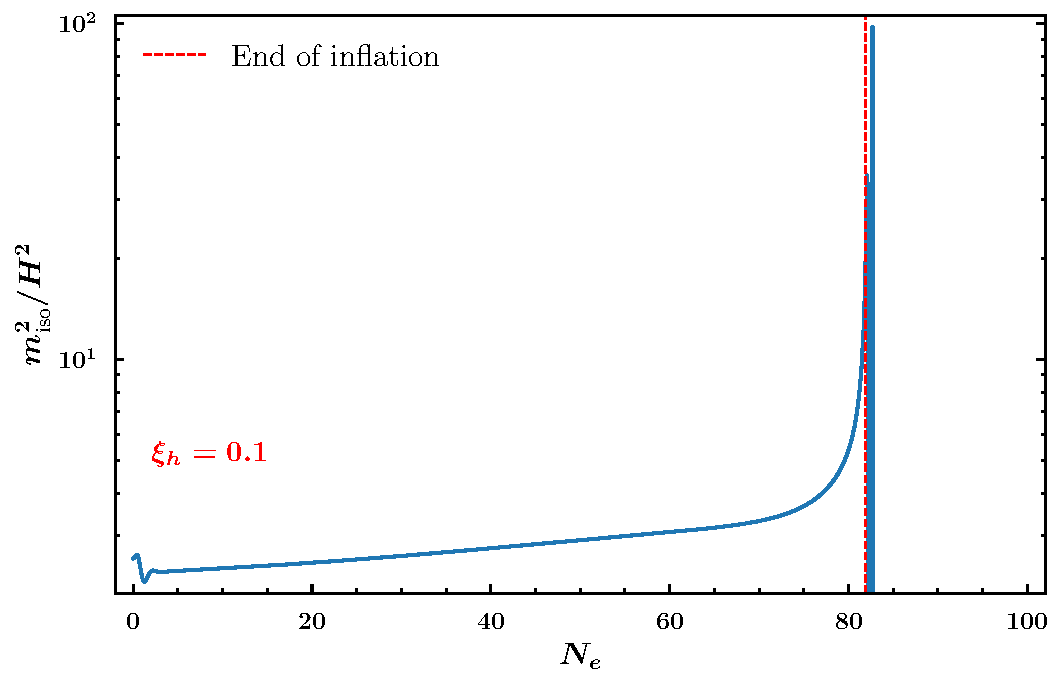
\includegraphics[width = 0.48 \textwidth]{Figures/isomass1.pdf}
    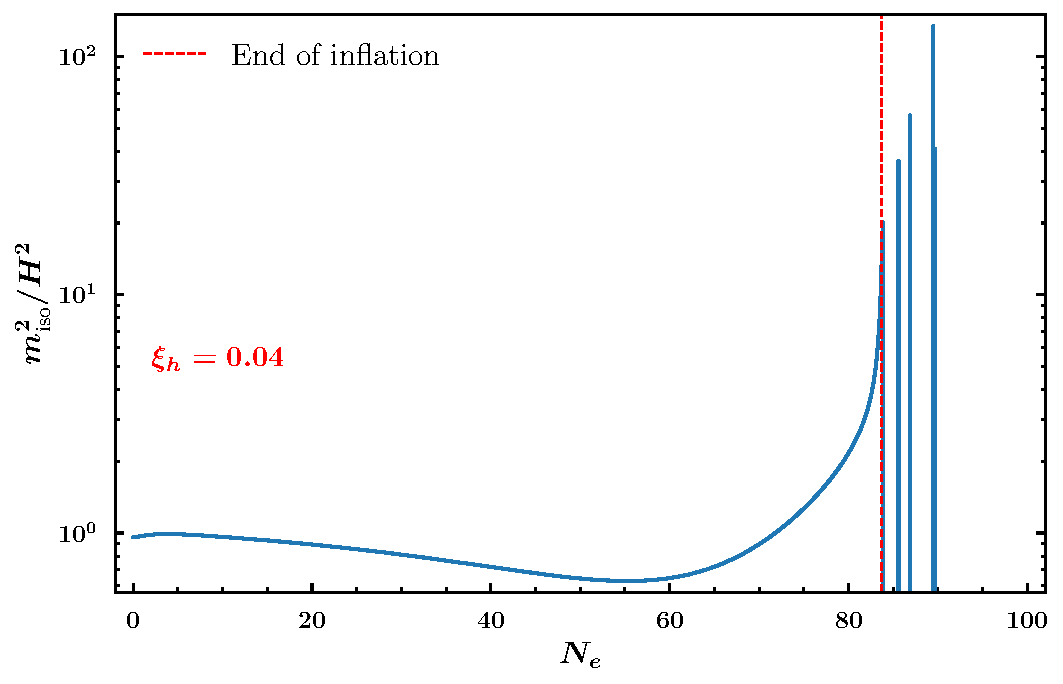
\includegraphics[width = 0.48 \textwidth]{Figures/isomass2.pdf}
    \caption{We show the isocurvature mass \eqref{iso mass} for a space of parameters that fulfill $\xi_h \sim \lambda \xi_s$ in function of number of e-folds $N_e$. In both panels we set $\lambda = 10^{-10}$ and $\xi_s = 4\times 10^{8}$}
    \label{fig3}
\end{figure}

Sin embargo, para un tratamiento completo que permita seguir la evolución completa de los modos $Q_s$ y $\mathcal{R}_k$, conviene adoptar un análisis numérico de las perturbaciones. Como en el caso del background, es más eficiente integrar numéricamente las ecuaciones \eqref{R ec.} y \eqref{Qs ec.} en términos de $N_e$:

\beq
    \mathcal{R}''_k + (3 + \epsilon - 2\eta_{||})\mathcal{R}'_k + \left(\dfrac{k}{aH}\right)^2 \mathcal{R}_k = -\dfrac{2\eta_\perp}{\sqrt{2\epsilon}}[Q_s' + (3-\xi_\perp - \eta_{||})Q_s]\,,
\enq


\beq
    Q_s'' + (3-\epsilon)Q_s' + \left[\left(\dfrac{k}{aH}\right)^2 + \dfrac{m_\text{iso}^2}{H^2} \right]Q_s = 2\sqrt{2\epsilon}\, \eta_\perp\mathcal{R}'_k\,,
\enq

donde $m_\text{iso}^2 = m_\text{iso}^2(N_e)$, $H = H(N_e)$ y $\eta_\perp = \eta_\perp(N_e)$. En la próxima sección procedemos a resolver estas ecuaciones con condiciones iniciales tipo Bunch-Davies.





\subsection{Isocurvature mass}

La masa del modo de isocurvarura $Q_s$ juega un papel fundamental en el análisis y evolución de la perturbaciones, pues como hemos visto, los efectos multi-campo están presentes incluso si el bendig es cero. Analicemos detenidamente la expresión \eqref{iso mass}. Como hemos mencionado, tenemos 3 términos que contribuyen a la masa $m_\text{iso}^2$: el término usual del potencial $V_{NN}$, una contribución geométrica intrísteca del espacio de campos dado por $R_\text{fs}$ y una contribución del bending. El término $V_{NN}$ está dado explícitamente por \cite{He2018}

\begin{align}
   \nonumber V_{NN} &= N^I N^J \nabla_I V_J = N^I N^J(\partial_I \partial_J V - \Gamma^K{}_{IJ}\partial_K V) \\[0.3cm]
     &= \dfrac{1}{\dot{\sigma}^2}\left(e^{\alpha\phi}\dot{\phi}^2 V_{hh} + e^{-\alpha \phi}\dot{h}^2 V_{\phi\phi} - 2\dot{\phi}\,\dot{h}V_{h\phi} - \dfrac{\alpha}{2}(\dot{\phi}^2 V_\phi + 2\dot{\phi}\,\dot{h}V_h ) \right)\,,
    \label{usual mass term}
\end{align}


el cual depende de las derivadas del potencial \eqref{potential Einstein} y de la dinámica de fondo. Sin embargo, se puede simplificar consdierablemente si tomamos en cuenta el valley-approach \eqref{valley} y los resultados \eqref{valley approach}. Sustituyendo explícitamente la forma de $N^I$, el potencial y tomando en cuenta \eqref{valley}, obtenemos

\beq
    V_{NN} \simeq \dfrac{\xi_h(24\lambda\xi_s + \xi_h(1 + 6\xi_h))}{\lambda\xi_s}\,H^2\,.
\enq 


En esta aproximación, la masa \eqref{iso mass} resulta 

\beq
    \dfrac{m_\text{iso}^2}{H^2} \simeq \dfrac{\xi_h(24\lambda\xi_s + \xi_h(1 + 6\xi_h))}{\lambda\xi_s} -\dfrac{\epsilon}{3} - \dfrac{\tilde{\xi}^2}{1 + \tilde{\xi}^2}\,,
\enq

donde $\tilde{\xi}^2 = \xi_h/6(\xi_h^2 + 4\lambda\xi_s)$. Podemos observar que en valley- approach, la masa del modo $Q_s$ toma una forma simplificada, y la razón $m_\text{iso}^2/H^2$ es constante. Esto puede ayudar a la búsqueda de soluciones analíticas de las ecuación para $Q_s$. Por otro lado, si $\xi_h \gg 1$, el modo de isocurvatura es pesado y el bending es despreciable, por lo que se puede ignorar la evolución de $Q_s$. Si tomamos $\xi_h \sim \lambda\xi_s$, el valor de $m_\text{iso}^2 $ es cercano a $H^2$, consecuentemente el modo $Q_s$ se vuelve ligero y el bending se vuelve significante. En este escenario, la aproximación single-field falla y se debe adoptar un escenario quasi-single field inflation \cite{Chen_2010,chen2010prd}, o resolver numéricamente las ecuaciones de los modos $\mathcal{R}_k$, $Q_s$, yendo más allá de la aproximación single-field slow roll \cite{Wang2017}.




\section{Isocurvature perturbations}
\label{{sec. 4}}

En esta sección mostramos los resultados analíticos y numéricos de la evolución del modo $Q_s$ y $\mathcal{R}_k$, tomando en cuenta los efectos multi-campo a través de la masa $m_\text{iso}^2$ y del bending $\eta_\perp$. Procedemos a resolver las ecuaciones \eqref{R ec.} ,\eqref{Qs ec.} en dos escenarios: para geodesic motion $\eta_\perp = 0$ y para el caso donde el bending es del orden de $\eta_\perp \sim \mathcal{O}(10^{-1})$. El primer caso se puede resolver analíticamente, pues las perturbaciones evolucionan de manera independiente a orden lineal. 




\subsection{Geodesic motion}

For geodesic motions $\eta_\perp = 0$, both modes decouple, so the $Q_s$ modes cannot transfer power to the $\mathcal{R}_k$ adiabatic modes, making it easier to find analytical solutions. Bajo la aproximación slow-roll y tomando 




\subsection{Numerical results}




\section{CMB observables}

\section{Discussion and conclusions}

\section{Acknowledgments}




\appendix

\section{Single-field inflation along the valleys 
\label{appendix1}}

La aproximación de los valles del potencial \eqref{potential Einstein} en el marco de Einstein es relevante para el análisis de la evolución de los campos $(\phi\,,h)$. En los trabajos previos sobre este modelo se discute este análisis con más detalle \cite{Wang2017,GUNDHI2020,He2018}, por lo que aquí nos limitaremos a presentar las ideas principales. En el límite $h\gg v_\text{ew}$, los valles del potencial \eqref{potential Einstein} están dados por la condición

\beq
\dfrac{\partial V}{\partial h} = 0\,,\quad h_0^2(\phi) = \dfrac{\xi_h}{\xi_h^2 + 4\lambda \xi_s}(e^{\alpha \phi} - 1 )
\label{valley}
\enq 

Esta condición sirve como un punto estacionario en el plano $(h\,,\dot{h})$; el escalarón $\phi$ rueda al mínimo del potencial \eqref{potential Einstein}, y por tanto los valles sirven como un atractor universal. Como el potencial es simétrico respecto a $h\to - h$, \eqref{valley} localiza los dos valles de $V(\phi\,,h)$. A lo largo de uno de los valles, el potencial está dado por el siguiente potencial efectivo en función de $\phi$

\beq 
    V_\text{eff}(\phi\,,h_0(\phi)) = \dfrac{ \lambda}{4(\xi_h^2 + 4\lambda\xi_s)}(1 - e^{-\alpha\phi})^2\,.
    \label{effective potential}
\enq 

Este potencial tiene exactamente la misma forma que el potencial del modelo de inflación $R^2$ o del modelo de Higgs \cite{BEZRUKOV2008}. Para el espacio estándar de parámetros discutido anteriormente, el modelo se reduce efectivamente a un modelo de un solo campo escalar. Dado que el campo de Higgs a lo largo de los valles está dado por \eqref{valley}, la acción \eqref{Higgs-R2 action} a lo largo de los valles toma la forma  

\beq
    S_E[g_\mu\,,\phi\,,h] = \int \dif^4 x\,\sqrt{-g}\,\left[\dfrac{1}{2}R - \dfrac{1}{2}g^{\mu\nu}\partial_\mu\phi\partial_\nu\phi \left(1 + \gamma^2(1 - e^{-\alpha\phi})^{-1}\right) -V_\text{eff}(\phi)\right]\,,
\enq 

donde $\tilde{\xi}^2 = \dfrac{\xi_h}{6(\xi_h^2 + 4\lambda\xi_s)}$. Vemos que si $\lambda = 0.13$, $\xi_h \sim 10^4$ la constante es del orden de $\tilde{\xi} \sim 10^{-5}$, por lo que el segundo factor del término cinético es subdominante. En la escala de inflación $\phi \gg 1$, el modelo se reduce efectivamente a la inflación canónica de un campo escalar con potencial efectivo dado por \eqref{effective potential}.  Sin embargo, para un espacio de parámetros tal que $\xi_h \sim \lambda\xi_s$ con la normalización \eqref{CMB constraint} fija, la constante resulta $\tilde{\xi}\sim \mathcal{O}(1)$. Este caso corresponde a lo que se conoce como quasi-single field inflation regimen \cite{chen2010prd,Chen_2010}.


A lo largo de los valles, tanto los vectores unitarios como el bending adoptan una forma simplficada

\beq 
    T^I = \dfrac{(1\,, \tilde{\xi} e^{\alpha\phi/2})}{\sqrt{1 + \tilde{\xi}^2}}\,,\quad N^I = \dfrac{(-\tilde{\xi}\,,  e^{\alpha\phi/2})}{\sqrt{1 + \tilde{\xi}^2}}\,, \quad \eta_\perp = \dfrac{\tilde{\xi}}{\sqrt{1 + \tilde{\xi}^2}}
    \label{valley approach}
\enq

Si $\tilde{\xi} \ll 1$, el vector $T^I$ apunta a la dirección de $\phi$, mientras que $N^I$ apunta en la dirección de $h$. El bending $\eta_\perp$ es despreciable dentro de los valles. 





%Bibliography

\bibliographystyle{abbrv}
\bibliography{main.bib}



\end{document}
